\documentclass[12pt]{article}
\usepackage{amsfonts}
\usepackage[normalem]{ulem}
\usepackage{graphicx}
\usepackage{enumitem}
\usepackage{ragged2e}
\usepackage{setspace}
\usepackage{tabto}
\usepackage{float}
\usepackage[hidelinks]{hyperref}
\usepackage{flowchart}\usepackage[paperheight=11.69in,paperwidth=8.27in,left=0.79in,right=0.79in,top=0.79in,bottom=0.79in,headheight=1in]{geometry}

%%%%%%%%%%%%%%%%%%%% Document code starts here %%%%%%%%%%%%%%%%%%%%

\begin{document}

\vspace{\baselineskip}

\vspace{\baselineskip}
{\fontsize{21.pt}{32.4pt}\selectfont \textbf{SUMMER INTERNSHIP }\par}\par
{\fontsize{21.pt}{32.4pt}\selectfont \textbf{ PROJECT REPORT   }\par}\par

\vspace{\baselineskip}
\vspace{\baselineskip}
{\fontsize{21pt}{25.2pt}\selectfont \textbf{INDIAN INSTITUTE OF TECHNOLOGY,} \par}\par
{\fontsize{21pt}{25.2pt}\selectfont \textbf{ HYDERABAD.}\par}\par

{\fontsize{21pt}{25.2pt}\selectfont (15/05/18-13/07/18)\par}\par


\vspace{\baselineskip}
{\fontsize{17pt}{20.4pt}\selectfont PROJECT TITLE\par}\par


\vspace{\baselineskip}
{\fontsize{20.74pt}{26.4pt}\selectfont \textbf{ARDUINO IN SCIENCE}\par}\par
{\fontsize{20.74pt}{26.4pt}\selectfont 1.)Accleration Due to gravity by Free fall\par}\par
{\fontsize{20.74pt}{26.4pt}\selectfont 2.)Speed of Sound Using Ultrasonic Sensor\par}\par
{\fontsize{20.74pt}{26.4pt}\selectfont 3.)RC circuit analysis\par}\par


\vspace{\baselineskip}

\vspace{\baselineskip}
{\fontsize{17.28pt}{19.2pt}\selectfont Supervisor,\par}\par


\vspace{\baselineskip}
{\fontsize{24.88pt}{28.8pt}\selectfont \textbf{Dr. G.V.V. Sharma,}\par}\par

{\fontsize{24.88pt}{28.8pt}\selectfont \textbf{Department of electrical engineering,}\par}\par

{\fontsize{24.88pt}{28.8pt}\selectfont \textbf{IIT Hyderabad.}\par}\par

\vspace{\baselineskip}

\vspace{\baselineskip}
{\fontsize{17.28pt}{19.2pt}\selectfont SUBMITTED BY,\par}\par

\vspace{\baselineskip}
{\fontsize{20.74pt}{24.0pt}\selectfont \textbf{PIYUSH PALIWAL,}\par}\par

{\fontsize{20.74pt}{24.0pt}\selectfont \textbf{BS-MS 2017,}\par}\par

{\fontsize{20.74pt}{24.0pt}\selectfont \textbf{IISER BHOPAL.}\par}\par

 %%%%%%%%%%%%  Starting New Page here %%%%%%%%%%%%%%
\newpage

{\fontsize{17.28pt}{19.2pt}\selectfont \textbf{ACKNOWLEDGEMENT}\par}\par

\vspace{\baselineskip}
{\fontsize{17.28pt}{19.2pt}\selectfont I am very thankful to IIT Hyderabad for giving me opportunity to undertake my summer internship at it’s electrical engineering department. It was very good learning experience for me to be intern here.\par}\par

\vspace{\baselineskip}
{\fontsize{17.28pt}{19.2pt}\selectfont I would like to convey my heartiest thanks to Dr. G.V.V. Sharma, for giving me proper guidance and opportunity of doing summer internship. I would like to thank to all teaching assistants who helped me during my internship. Also I would like to thank Mr. Velumurugan, technician at EE lab who assisted and guided me whenever I needed. I would like to thank Mr. Hanumant and Mr. Swaroop Reddy for their guidance.\par}\par


\vspace{\baselineskip}
{\fontsize{17.28pt}{19.2pt}\selectfont I am extremely thankful to IIT Hyderabad for providing me facilities to work in, with out which this work would not be possible.\par}\par


\vspace{\baselineskip}
{\fontsize{17.28pt}{19.2pt}\selectfont Last but not the least; I would like to thank all the staff of IIT Hyderabad, for being so helpful during this summer internship.\par}\par


\vspace{\baselineskip}
{\fontsize{17.28pt}{19.2pt}\selectfont  \par}

 %%%%%%%%%%%%  Starting New Page here %%%%%%%%%%%%%%

\newpage
\par

{\fontsize{17.28pt}{19.2pt}\selectfont \textbf{Preface}\par}\par


\vspace{\baselineskip}
{\fontsize{17.28pt}{19.2pt}\selectfont   Objective of this project was how to make SCIENCE experiments more interesting using Arduino microcontroller.Arduino is Open-source electronic prototyping platform enabling users to create interactive electronic objects.. All things one need to know is basic circuits and little bit coding. In this project first part I have made experiments setup for determining value of \textbf{g}(acceleration due to gravity) by getting time of travel of freely falling object using photo interrupter and piezo electric sensors. In second part of project speed of sound is determined by using ultrasonic sensor. In this part I have connected clap switch with it to activate transmitter and receiver of ultrasonic sensor to detect time of travel of sound wave. In third part of project, I have done RC circuit analysis. In this part, charging and discharging of capacitor with time is observed and it’s graph is obtained. \par}\par


\vspace{\baselineskip}
{\fontsize{17.28pt}{19.2pt}\selectfont This project shows some applications of Arduino in designing experimental setups of science experiments by own. By this project we get an idea how interesting it is when we understand science by our own designed experiments. Main goal of this project was to understand the science with help of engineering just like $"$learning by doing it$"$.\par}\par

{\fontsize{17.28pt}{19.2pt}\selectfont \textbf{\tab \  }\par}

 %%%%%%%%%%%%  Starting New Page here %%%%%%%%%%%%%%

\newpage
\par


\vspace{\baselineskip}
\tab \tab \tab \tab \tab {\fontsize{14pt}{16.8pt}\selectfont \textbf{\uline{ARDUINO IN SCIENCE}}\par}\par


\vspace{\baselineskip}
{\fontsize{14pt}{16.8pt}\selectfont \textbf{1.)\ \  Experimental setup for determining value of acceleration due to gravity:}\par}\par


\vspace{\baselineskip}
{\fontsize{14pt}{16.8pt}\selectfont \textbf{OBJECTIVE:}\  finding time of travel by the freely falling object to determine It’s acceleration.\par}\par


\vspace{\baselineskip}
{\fontsize{14pt}{16.8pt}\selectfont \textbf{COMPONENTS REQUIRED:}\par}\par

\begin{itemize}
	\item {\fontsize{14pt}{16.8pt}\selectfont Arduino UNO\par}\par

	\item {\fontsize{14pt}{16.8pt}\selectfont 4 - piezo electric sensors\par}\par

	\item {\fontsize{14pt}{16.8pt}\selectfont 1 - photo interrupter\par}\par

	\item {\fontsize{14pt}{16.8pt}\selectfont 1-LED\par}\par

	\item {\fontsize{14pt}{16.8pt}\selectfont 4-resisters(1k ohm)\par}\par

	\item {\fontsize{14pt}{16.8pt}\selectfont two boxes\par}
\end{itemize}\par


\vspace{\baselineskip}
{\fontsize{14pt}{16.8pt}\selectfont \textbf{CONNECTIONS:}\par}\par


\vspace{\baselineskip}
\begin{itemize}
	\item {\fontsize{14pt}{16.8pt}\selectfont photo interrupter has three pins: GND, VCC, OUT\par}\par

{\fontsize{14pt}{16.8pt}\selectfont connect GND to GND of Arduino, VCC to 5V of Arduino, OUT to A4 of Arduino\par}\par

	\item {\fontsize{14pt}{16.8pt}\selectfont we have 4 piezo electric sensors. Connect positive terminal to one end of 1k ohm resister and negative to ground of Arduino. Connect other end of resister to negative of piezo electric sensor. Connect pin A0 of Arduino to positive terminal of piezo-electric sensor.\par}\par

	\item {\fontsize{14pt}{16.8pt}\selectfont Make similar connections for other piezo electric sensors and connect their positive terminals to A1, A2, A3 of Arduino.\par}\par

	\item {\fontsize{14pt}{16.8pt}\selectfont Connect LED: positive to digital pin 13 of Arduino and negative to ground.\par}
\end{itemize}\par


\vspace{\baselineskip}

\vspace{\baselineskip}
{\fontsize{14pt}{16.8pt}\selectfont \textbf{PREPARTION OF SETUP:}\par}\par

\begin{itemize}
	\item {\fontsize{14pt}{16.8pt}\selectfont In one box fix photo interrupter sensor. On other box fix 4-piezo electric sensors and cover them with card board so that when object will fall on card board piezo sensor can detect it and send signal to Arduino.\par}\par

	\item {\fontsize{14pt}{16.8pt}\selectfont The box having piezo electric sensor is kept at ground and box containing photo interrupter is kept on the top of the table. Make sure that the gap of photo interrupter should of exactly on the piezo sensors so that when object will pass through this gap,it directly falls on piezo sensors.\par}\par

	\item {\fontsize{14pt}{16.8pt}\selectfont After preparation of setup and connections, now connect Arduino to computer and upload the Arduino code which is given after circuit diagram\par}
\end{itemize}\par

\vspace{\baselineskip}
{\fontsize{14pt}{16.8pt}\selectfont \textbf{FORMULA:}\par}\par

\vspace{\baselineskip}
{\fontsize{14pt}{16.8pt}\selectfont From equation of motion of particle in straight line,\par}\par

\vspace{\baselineskip}
{\fontsize{14pt}{16.8pt}\selectfont  d=$V$\textsubscript{0} t+ (1/2) a$t$\textsuperscript{2}. \par}\par

{\fontsize{14pt}{16.8pt}\selectfont for freely falling object with $V$\textsubscript{0}=0 has a=(2d)/$t$\textsuperscript{2}. And this a=g\par}\par

\vspace{\baselineskip}

\vspace{\baselineskip}
{\fontsize{14pt}{16.8pt}\selectfont \textbf{CIRCUIT DIAGRAM:}\par}\par

\vspace{\baselineskip}
{\fontsize{14pt}{16.8pt}\selectfont Connections of piezo electric sensors and photo interrupter with Arduino.\par}\par

\vspace{\baselineskip}

%%%%%%%%%%%%%%%%%%%% Figure/Image No: 1 starts here %%%%%%%%%%%%%%%%%%%%

\begin{figure}[H]
	\begin{Center}
		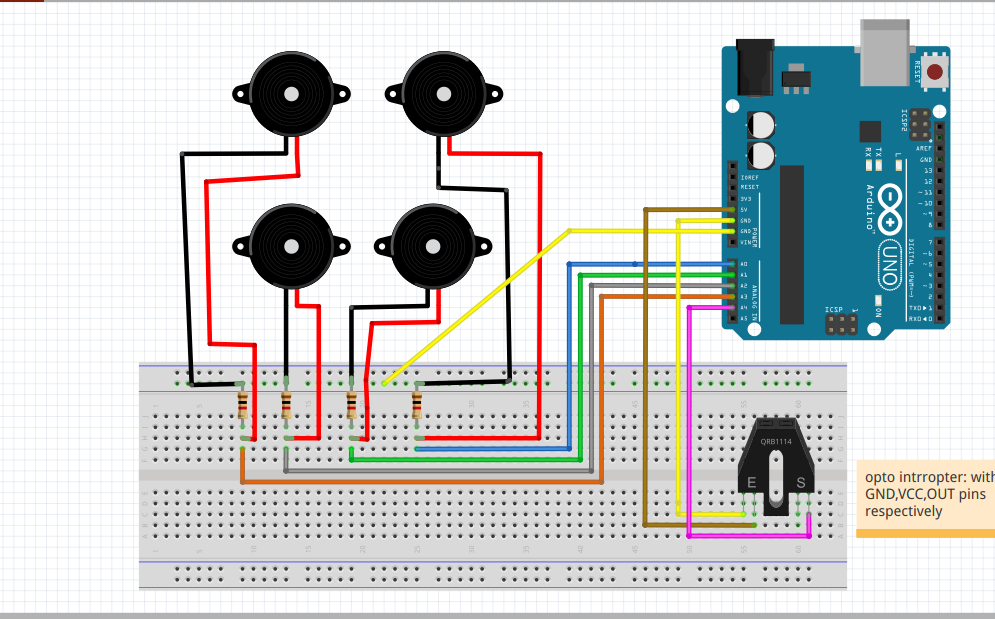
\includegraphics[width=6.69in,height=4.16in]{./media/image1.png}
	\end{Center}
\end{figure}


%%%%%%%%%%%%%%%%%%%% Figure/Image No: 1 Ends here %%%%%%%%%%%%%%%%%%%%

\vspace{\baselineskip}
{\fontsize{14pt}{16.8pt}\selectfont \textbf{ARDUINO CODE:}\par}\par

\vspace{\baselineskip}
{\fontsize{14pt}{16.8pt}\selectfont const int ledPin= 13;\par}\par

{\fontsize{14pt}{16.8pt}\selectfont const int threshold=1;\par}\par

{\fontsize{14pt}{16.8pt}\selectfont long int endTime=0,startTime=0;\par}\par

{\fontsize{14pt}{16.8pt}\selectfont double Time;\par}\par

{\fontsize{14pt}{16.8pt}\selectfont float\ d=0.9;  //hight of photointerrupter from piezosensors\par}\par

{\fontsize{14pt}{16.8pt}\selectfont int count=0;\par}\par


\vspace{\baselineskip}
{\fontsize{14pt}{16.8pt}\selectfont void setup()\par}\par

{\fontsize{14pt}{16.8pt}\selectfont $ \{ $ \par}\par

{\fontsize{14pt}{16.8pt}\selectfont \  Serial.begin(9600);\par}\par

{\fontsize{14pt}{16.8pt}\selectfont \  pinMode(ledPin, OUTPUT);\par}\par

{\fontsize{14pt}{16.8pt}\selectfont \  \par}\par

{\fontsize{14pt}{16.8pt}\selectfont $ \} $ \par}\par


\vspace{\baselineskip}
{\fontsize{14pt}{16.8pt}\selectfont void loop()\par}\par

{\fontsize{14pt}{16.8pt}\selectfont $ \{ $ \par}\par

{\fontsize{14pt}{16.8pt}\selectfont \  int\ val=\ analogRead(A0);   //analogpin connected to piezosensor-1\par}\par

{\fontsize{14pt}{16.8pt}\selectfont \  int\ val2=analogRead(A1);\   //piezosensor-2\par}\par

{\fontsize{14pt}{16.8pt}\selectfont \  int\ val3=analogRead(A2);\   //piezosensor-3\par}\par

{\fontsize{14pt}{16.8pt}\selectfont \  int\ val4=analogRead(A3);\   //piezosensor-4\par}\par

{\fontsize{14pt}{16.8pt}\selectfont \  int\ val5=analogRead(A4);\   //analogpin connected to photointerrupter\par}\par

{\fontsize{14pt}{16.8pt}\selectfont \  Serial.print(val);\tab \ \ \ \ \ \ \ \ \ \ \ // printing  values of each sensor on serial monitor\par}\par

{\fontsize{14pt}{16.8pt}\selectfont \  Serial.print(" ");\par}\par

{\fontsize{14pt}{16.8pt}\selectfont \  Serial.print(val2);\par}\par

{\fontsize{14pt}{16.8pt}\selectfont \  Serial.print(" ");\par}\par

{\fontsize{14pt}{16.8pt}\selectfont \  Serial.print(val3);\par}\par

{\fontsize{14pt}{16.8pt}\selectfont \  Serial.print(" ");\par}\par

{\fontsize{14pt}{16.8pt}\selectfont \  Serial.print(val4);\par}\par

{\fontsize{14pt}{16.8pt}\selectfont \  Serial.print(" ");\par}\par

{\fontsize{14pt}{16.8pt}\selectfont \  Serial.println(val5);\par}\par


\vspace{\baselineskip}
{\fontsize{14pt}{16.8pt}\selectfont \  if(val5 \textgreater 1000)\ \  //when some object come in between interrupter analog pin becomes high\par}\par

{\fontsize{14pt}{16.8pt}\selectfont \  $ \{ $ \par}\par

{\fontsize{14pt}{16.8pt}\selectfont \ \ \  startTime=millis();\par}\par

{\fontsize{14pt}{16.8pt}\selectfont \  $ \} $ \par}\par

{\fontsize{14pt}{16.8pt}\selectfont  if (val\textgreater=threshold$ \vert $ $ \vert $ val2\textgreater=threshold$ \vert $ $ \vert $ \par}\par
{\fontsize{14pt}{16.8pt}\selectfont val3\textgreater=threshold$ \vert $ $ \vert $ val4\textgreater=threshold)\par}\par

{\fontsize{14pt}{16.8pt}\selectfont \  $ \{ $ \par}\par

{\fontsize{14pt}{16.8pt}\selectfont \ \  endTime=millis();\par}\par

{\fontsize{14pt}{16.8pt}\selectfont \ \  Serial.print("EndTime : ");\par}\par

{\fontsize{14pt}{16.8pt}\selectfont \ \  Serial.print((float)endTime/1000);\par}\par

{\fontsize{14pt}{16.8pt}\selectfont \ \  Serial.print(" ");\par}\par

{\fontsize{14pt}{16.8pt}\selectfont \ \  Serial.print("StartTime : ");\par}\par

{\fontsize{14pt}{16.8pt}\selectfont \ \  Serial.println((float)startTime/1000);\par}\par

{\fontsize{14pt}{16.8pt}\selectfont \ \  Serial.print("Time Of Flight : ");\par}\par

{\fontsize{14pt}{16.8pt}\selectfont \ \  Time=(float)(endTime-startTime)/1000;\par}\par

{\fontsize{14pt}{16.8pt}\selectfont \ \  Serial.println(Time);\par}\par

{\fontsize{14pt}{16.8pt}\selectfont \ \  Serial.print("Acceleration of particle : ");.\par}\par

{\fontsize{14pt}{16.8pt}\selectfont \ \  Serial.println((d$\ast$ 2.0)/(Time$\ast$ Time));\par}\par

{\fontsize{14pt}{16.8pt}\selectfont \  \par}\par

{\fontsize{14pt}{16.8pt}\selectfont \  digitalWrite(ledPin,\ HIGH);  // LED glowing\par}\par

{\fontsize{14pt}{16.8pt}\selectfont \  delay(3000);\par}\par

{\fontsize{14pt}{16.8pt}\selectfont \  digitalWrite(ledPin, LOW);\par}\par

{\fontsize{14pt}{16.8pt}\selectfont \  delay(5000);\par}\par

{\fontsize{14pt}{16.8pt}\selectfont \  $ \} $ \par}\par

{\fontsize{14pt}{16.8pt}\selectfont \  else\par}\par

{\fontsize{14pt}{16.8pt}\selectfont \  $ \{ $ \par}\par

{\fontsize{14pt}{16.8pt}\selectfont \  digitalWrite(ledPin, LOW);\par}\par

{\fontsize{14pt}{16.8pt}\selectfont \  $ \} $ \par}\par

{\fontsize{14pt}{16.8pt}\selectfont \  delay(1);\par}\par

{\fontsize{14pt}{16.8pt}\selectfont $ \} $ \par}\par

\vspace{\baselineskip}

\vspace{\baselineskip}
{\fontsize{14pt}{16.8pt}\selectfont \textbf{OBSERVATION:}\par}\par

\vspace{\baselineskip}
{\fontsize{14pt}{16.8pt}\selectfont After uploading code, now open serial monitor and observe values of each sensor detecting. Now leave object from gap of photo interrupter and observe serial monitor. It will print the acceleration of the object.\par}\par


\vspace{\baselineskip}
{\fontsize{14pt}{16.8pt}\selectfont \textbf{RESULT:}\par}\par


\vspace{\baselineskip}
{\fontsize{14pt}{16.8pt}\selectfont Using this setup acceleration of freely falling object can be determined easily. And the result I got was in between 9-10 m/$s$\textsuperscript{2}\  which is near to exact value 9.81 m/$s$\textsuperscript{2}.\par}

 %%%%%%%%%%%%  Starting New Page here %%%%%%%%%%%%%%

\newpage
\par

\vspace{\baselineskip}
{\fontsize{14pt}{16.8pt}\selectfont \textbf{2.) Measurement of speed of sound using ultrasonic sensor and it’s activation using clap switch}\par}\par

\vspace{\baselineskip}
{\fontsize{14pt}{16.8pt}\selectfont \textbf{OBJECTIVE:} measuring speed of sound. Making and using clap switch.\par}\par

\vspace{\baselineskip}
{\fontsize{14pt}{16.8pt}\selectfont \textbf{COMPONENTS: }\par}\par

\begin{itemize}
	\item {\fontsize{14pt}{16.8pt}\selectfont Arduino UNO\par}\par

	\item {\fontsize{14pt}{16.8pt}\selectfont Ultrasonic sensor\par}\par

	\item {\fontsize{14pt}{16.8pt}\selectfont LCD (16x2)\par}\par

	\item {\fontsize{14pt}{16.8pt}\selectfont Electret microphone\par}\par

	\item {\fontsize{14pt}{16.8pt}\selectfont 15k ohm – 2 resister\par}\par

	\item {\fontsize{14pt}{16.8pt}\selectfont 1M ohm – 1 resister\par}\par

	\item {\fontsize{14pt}{16.8pt}\selectfont 1k ohm -1 resister\par}\par

	\item {\fontsize{14pt}{16.8pt}\selectfont 1 LED\par}\par

	\item {\fontsize{14pt}{16.8pt}\selectfont 1-Capacotor (100 micro F)\par}\par

	\item {\fontsize{14pt}{16.8pt}\selectfont 2-capacitor(100nF)\par}\par

	\item {\fontsize{14pt}{16.8pt}\selectfont 2N3904 NPN transistor\par}
\end{itemize}\par

\vspace{\baselineskip}
{\fontsize{14pt}{16.8pt}\selectfont \textbf{CIRCUIT DIAGRAM:}\par}\par

\vspace{\baselineskip}

%%%%%%%%%%%%%%%%%%%% Figure/Image No: 2 starts here %%%%%%%%%%%%%%%%%%%%
\begin{figure}[H]
\advance\leftskip -0.53in	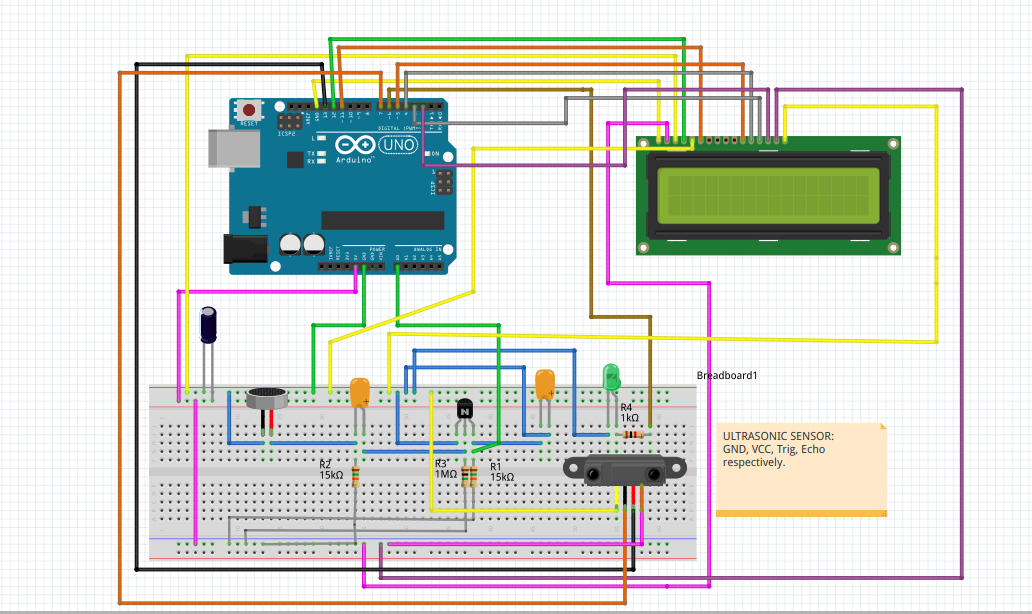
\includegraphics[width=6.5in,height=4.0in]{./media/image2.png}
\end{figure}

%%%%%%%%%%%%%%%%%%%% Figure/Image No: 2 Ends here %%%%%%%%%%%%%%%%%%%%

{\fontsize{14pt}{16.8pt}\selectfont connection of ultrasonic sensor, clap switch and LCD to Arduino UNO. \tabto{5.98in} \par}\par

\vspace{\baselineskip}
\vspace{\baselineskip}

\vspace{\baselineskip}
{\fontsize{14pt}{16.8pt}\selectfont \textbf{PERPARATION OF SETUP:}\par}\par

\vspace{\baselineskip}
{\fontsize{14pt}{16.8pt}\selectfont After making connection according to circuit diagram keep ultrasonic sensor against some barrier at measured distance and note this distance of barrier from sensor. Use this fixed distance in code of Arduino.\par}\par

\vspace{\baselineskip}
{\fontsize{14pt}{16.8pt}\selectfont After preparing setup, upload following code to Arduino board.\par}\par

\vspace{\baselineskip}
{\fontsize{14pt}{16.8pt}\selectfont \textbf{ARDUINO CODE:}\par}\par

\vspace{\baselineskip}
{\fontsize{14pt}{16.8pt}\selectfont $\#$ include<LiquidCrystal.h>\par}\par

{\fontsize{14pt}{16.8pt}\selectfont LiquidCrystal lcd(12,11,5,4,3,2);\par}\par

{\fontsize{14pt}{16.8pt}\selectfont int sensorValue = 0,sensorValue1=0;\par}\par

{\fontsize{14pt}{16.8pt}\selectfont int trigPin=13,echoPin=7;\par}\par

{\fontsize{14pt}{16.8pt}\selectfont int\ distance=60;\   // fixed distance in my case is 60cm. \par}\par

{\fontsize{14pt}{16.8pt}\selectfont int p=0,time;\par}\par

{\fontsize{14pt}{16.8pt}\selectfont void setup() \par}\par

{\fontsize{14pt}{16.8pt}\selectfont $ \{ $ \par}\par

{\fontsize{14pt}{16.8pt}\selectfont \  lcd.begin(16,2);\par}\par

{\fontsize{14pt}{16.8pt}\selectfont \  lcd.setCursor(0,0);\par}\par

{\fontsize{14pt}{16.8pt}\selectfont \  lcd.print("Setup is ready");\par}\par

{\fontsize{14pt}{16.8pt}\selectfont \  pinMode(6,OUTPUT);\par}\par

{\fontsize{14pt}{16.8pt}\selectfont \  pinMode(trigPin,OUTPUT);\par}\par

{\fontsize{14pt}{16.8pt}\selectfont \  pinMode(echoPin,INPUT);\par}\par

{\fontsize{14pt}{16.8pt}\selectfont \  Serial.begin(9600);\par}\par

{\fontsize{14pt}{16.8pt}\selectfont $ \} $ \par}\par

{\fontsize{14pt}{16.8pt}\selectfont void loop() \par}\par

{\fontsize{14pt}{16.8pt}\selectfont $ \{ $ \par}\par

{\fontsize{14pt}{16.8pt}\selectfont  sensorValue = analogRead(0); \par}\par

{\fontsize{14pt}{16.8pt}\selectfont  if(sensorValue>50)\  // when microphone sense sound of high intensity \par}\par

{\fontsize{14pt}{16.8pt}\selectfont \  $ \{ $ \par}\par

{\fontsize{14pt}{16.8pt}\selectfont \  digitalWrite(6,HIGH);\par}\par

{\fontsize{14pt}{16.8pt}\selectfont \  delay(1000);\par}\par

{\fontsize{14pt}{16.8pt}\selectfont \  digitalWrite(6,LOW);\par}\par

{\fontsize{14pt}{16.8pt}\selectfont \  delay(1000);\par}\par

{\fontsize{14pt}{16.8pt}\selectfont \  p++;\par}\par

{\fontsize{14pt}{16.8pt}\selectfont \  $ \} $ \par}\par

{\fontsize{14pt}{16.8pt}\selectfont \  if(p==1) // when clap switch becomes active then sensor becomes active \par}\par

{\fontsize{14pt}{16.8pt}\selectfont \  $ \{ $ \par}\par

{\fontsize{14pt}{16.8pt}\selectfont \ \ \  digitalWrite(trigPin,LOW);\par}\par

{\fontsize{14pt}{16.8pt}\selectfont \ \ \  delayMicroseconds(2000);\par}\par

{\fontsize{14pt}{16.8pt}\selectfont \ \ \  digitalWrite(trigPin,HIGH);\par}\par

{\fontsize{14pt}{16.8pt}\selectfont \ \ \  digitalWrite(trigPin,LOW);\par}\par

{\fontsize{14pt}{16.8pt}\selectfont \ \ \  time=pulseIn(echoPin,HIGH);\par}\par

{\fontsize{14pt}{16.8pt}\selectfont \ \ \  p=(double)time/1000000;\par}\par

{\fontsize{14pt}{16.8pt}\selectfont \ \  Serial.print("Speed of sound is :");\par}\par

{\fontsize{14pt}{16.8pt}\selectfont \ \  Serial.print((float)(distance$\ast$ 2)/(p$\ast$ 100));\par}\par

{\fontsize{14pt}{16.8pt}\selectfont \ \  Serial.println("m/s");\par}\par

{\fontsize{14pt}{16.8pt}\selectfont \ \  lcd.setCursor(0,0);\par}\par

{\fontsize{14pt}{16.8pt}\selectfont \ \  lcd.println("Velocity of sound");\par}\par

{\fontsize{14pt}{16.8pt}\selectfont \ \  lcd.setCursor(0,1);\par}\par

{\fontsize{14pt}{16.8pt}\selectfont \ \  lcd.print((float)(distance$\ast$ 2)/(p$\ast$ 100));\par}\par

{\fontsize{14pt}{16.8pt}\selectfont \ \  lcd.print(" ");\par}\par

{\fontsize{14pt}{16.8pt}\selectfont \ \  lcd.print("m/s");\par}\par

{\fontsize{14pt}{16.8pt}\selectfont \ \  delay(4000);\par}\par

{\fontsize{14pt}{16.8pt}\selectfont \ \  lcd.setCursor(0,0);\par}\par

{\fontsize{14pt}{16.8pt}\selectfont \ \  lcd.println("-setup is ready-");\par}\par

{\fontsize{14pt}{16.8pt}\selectfont \ \  lcd.setCursor(0,1);\par}\par

{\fontsize{14pt}{16.8pt}\selectfont \ \  lcd.println("\ \ \ \ \ \ \ \ \ \ \ \ \ \  ");\par}\par

{\fontsize{14pt}{16.8pt}\selectfont \ \  p=0;\par}\par

{\fontsize{14pt}{16.8pt}\selectfont \  $ \} $ \par}\par

{\fontsize{14pt}{16.8pt}\selectfont $ \} $ \par}\par

\vspace{\baselineskip}
{\fontsize{14pt}{16.8pt}\selectfont \textbf{FORMULA:}\par}\par

\vspace{\baselineskip}
{\fontsize{14pt}{16.8pt}\selectfont Ultrasonic sensor is emitting sound wave of frequency higher than 20kHz which can’t be detected by Human ears. Due to it’s high frequency it distorts less and gets reflected if some barrier comes in between transmitter. After reflecting, this wave is detected by receiver.\par}\par

\vspace{\baselineskip}
{\fontsize{14pt}{16.8pt}\selectfont Here we have fixed distance of barrier from transmitter and time taken by wave to come back to receiver is twice than time taken to travel fixed distance.\par}\par

\vspace{\baselineskip}
{\fontsize{14pt}{16.8pt}\selectfont Time of travel= (time detected by sensor)/2\par}\par

\vspace{\baselineskip}
{\fontsize{14pt}{16.8pt}\selectfont Speed = (fixed distance)/Time of travel.\par}\par

\vspace{\baselineskip}
{\fontsize{14pt}{16.8pt}\selectfont  Which is speed of sound.\par}\par

%working principal of clap switch circuit
\vspace{\baselineskip}
{\fontsize{14pt}{16.8pt}\selectfont \textbf {WORKING PRINCIPLE OF CLAP SWITCH CIRCUIT:}\par}\par 

\vspace{\baselineskip}
{\fontsize{14pt}{16.8pt}\selectfont  Clap switch circuit consists of filter circuit and amplifier. Electret microphone when detect presence of sound waves it sends elecrical signals to RC filter. RC filter removes noise from signals and send filtered signals to NPN transister. NPN transister amplifies signals it getting from RC filter and send it to analog pin of Arduino board where it's presence is detected and at appropriate signal strength, switch becomes active.\par}\par  


\vspace{\baselineskip}
{\fontsize{14pt}{16.8pt}\selectfont \textbf{OBSERVATION:}\par}\par

\vspace{\baselineskip}
{\fontsize{14pt}{16.8pt}\selectfont After uploading code, clap loudly. Due to clap, clap switch becomes active and it will turn ON Ultrasonic sensor and LCD display and start calculating speed of sound depending upon the time taken by ultrasonic sound wave to travel fixed distance.\par}\par

\vspace{\baselineskip}
{\fontsize{14pt}{16.8pt}\selectfont \textbf{RESULT:\ \ \ \  }Speed of sound measured using this setup is about 336 m/$s$\textsuperscript{2}.\ Which\ is\    closer to exact value 343m/$s$\textsuperscript{2}.\par}\par

\vspace{\baselineskip}
{\fontsize{14pt}{16.8pt}\selectfont \textbf{3.) analysis capacitor’s charging and discharging curve from data obtained by Arduino.}\par}\par

\vspace{\baselineskip}
{\fontsize{14pt}{16.8pt}\selectfont \textbf{OBJECTIVE: }analysis of charging and discharging values of voltages with time.\par}\par

\vspace{\baselineskip}
{\fontsize{14pt}{16.8pt}\selectfont \textbf{COMPONENTS:\ \  }\par}\par

\begin{itemize}
	\item {\fontsize{14pt}{16.8pt}\selectfont 10 M ohm resister\par}\par

	\item {\fontsize{14pt}{16.8pt}\selectfont Capacitor of 0.44 micro F ( use plastic film capacitor but don’t use electrolytic capacitor)\par}\par

	\item {\fontsize{14pt}{16.8pt}\selectfont Arduino UNO\par}
\end{itemize}\par

\vspace{\baselineskip}
{\fontsize{14pt}{16.8pt}\selectfont \textbf{CIRCUIT DIAGRAM:}\par}\par

\vspace{\baselineskip}

%%%%%%%%%%%%%%%%%%%% Figure/Image No: 3 starts here %%%%%%%%%%%%%%%%%%%%
\begin{figure}[H]
	\begin{Center}
		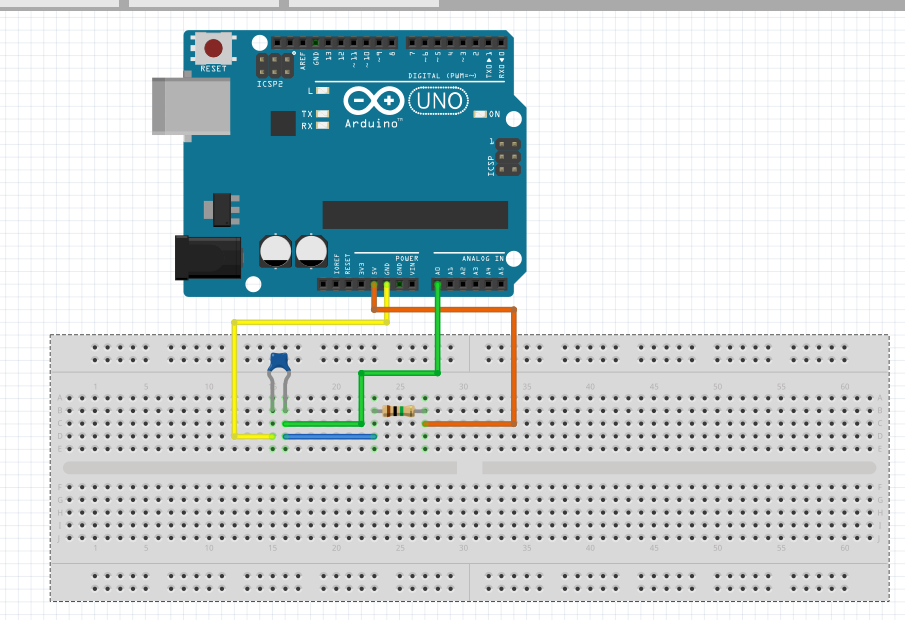
\includegraphics[width=6.69in,height=4.59in]{./media/image3.png}
	\end{Center}
\end{figure}
%%%%%%%%%%%%%%%%%%%% Figure/Image No: 3 Ends here %%%%%%%%%%%%%%%%%%%%

\par

\vspace{\baselineskip}
{\fontsize{14pt}{16.8pt}\selectfont After making connections according to circuit diagram, upload following code to Arduino.\par}\par

\vspace{\baselineskip}
{\fontsize{14pt}{16.8pt}\selectfont \textbf{ARDUINO CODE:} \par}\par

\vspace{\baselineskip}
{\fontsize{14pt}{16.8pt}\selectfont float v1=0;\par}\par

{\fontsize{14pt}{16.8pt}\selectfont void setup() $ \{ $ \par}\par

{\fontsize{14pt}{16.8pt}\selectfont \  Serial.begin(9600);\par}\par

{\fontsize{14pt}{16.8pt}\selectfont \  Serial.println("CLEARDATA");\par}\par

{\fontsize{14pt}{16.8pt}\selectfont \  Serial.println("LABEL,Computer Time,Time (Milli Sec.),Volt");\par}\par

\vspace{\baselineskip}
{\fontsize{14pt}{16.8pt}\selectfont $ \} $ \par}\par

\vspace{\baselineskip}
{\fontsize{14pt}{16.8pt}\selectfont void loop() $ \{ $ \par}\par

{\fontsize{14pt}{16.8pt}\selectfont \  v1=(float)5.0$\ast$ analogRead(A0)/1024.0;\par}\par

{\fontsize{14pt}{16.8pt}\selectfont \  Serial.print("DATA,TIME,");\par}\par

{\fontsize{14pt}{16.8pt}\selectfont \  Serial.print(millis());\par}\par

{\fontsize{14pt}{16.8pt}\selectfont \  Serial.print(",");\par}\par

{\fontsize{14pt}{16.8pt}\selectfont \  Serial.println(v1);\par}\par

{\fontsize{14pt}{16.8pt}\selectfont \  delay(100);\par}\par

{\fontsize{14pt}{16.8pt}\selectfont $ \} $ \par}\par

\vspace{\baselineskip}
{\fontsize{14pt}{16.8pt}\selectfont \textbf{HOW TO OBSERVE CHARGING AND DISCHARGING VALUES OF VOLTAGE:}\par}\par

\vspace{\baselineskip}
{\fontsize{14pt}{16.8pt}\selectfont After uploading code open serial monitor, we will observe values of voltage across capacitor on serial monitor.\par}\par

\vspace{\baselineskip}
{\fontsize{14pt}{16.8pt}\selectfont To observe charging value of voltage, first discharge capacitor by connecting it’s both ends and then connect it to circuit.\par}\par

\vspace{\baselineskip}
{\fontsize{14pt}{16.8pt}\selectfont To observe discharging value of voltage, disconnect 5V pin from Arduino after full charging of capacitor and connect extreme end of capacitor to another end of resister.\par}\par

\vspace{\baselineskip}
{\fontsize{14pt}{16.8pt}\selectfont This way we can observe charging and discharging values of voltage on serial monitor.\par}\par

\vspace{\baselineskip}
{\fontsize{14pt}{16.8pt}\selectfont \textbf{How to print charging and discharging values of voltage directly to MS EXCEL:}\par}\par

\vspace{\baselineskip}
{\fontsize{14pt}{16.8pt}\selectfont MS Excel provides features to connect serial monitor directly to excel sheet. It provides better way to analyse data we are getting from Arduino and obtain results quickly.\par}\par

\vspace{\baselineskip}
{\fontsize{14pt}{16.8pt}\selectfont For that we need to install $``$PLX-DAQ$"$  in our windows.\par}\par

\vspace{\baselineskip}
{\fontsize{14pt}{16.8pt}\selectfont We can refer following links to know how to install and use \textbf{$``$PLX-DAQ$"$ }:\par}\par

\vspace{\baselineskip}

\vspace{\baselineskip}
{\fontsize{14pt}{16.8pt}\selectfont \ \ \ \ \ \  To install $``$PLX-DAQ$"$  refer: \href{https://www.parallax.com/downloads/plx-daq}{https://www.parallax.com/downloads/plx-daq}\par}\par

\vspace{\baselineskip}
{\fontsize{14pt}{16.8pt}\selectfont \ \ \ \ \  To know how to connect PLX-DAQ to excel refer: \par}\par

{\fontsize{14pt}{16.8pt}\selectfont \ \ \ \ \ \  \href{https://medium.com/@islamnegm/quick-start-to-simple-daq-system-using-plx-daq-excel-arduino-d2457773384b}{https://medium.com/@islamnegm/quick-start-to-simple-daq-system-using-plx-daq-excel-arduino-d2457773384b}\par}

 %%%%%%%%%%%%  Starting New Page here %%%%%%%%%%%%%%
\newpage
\par

{\fontsize{14pt}{16.8pt}\selectfont \textbf{FORMULA:}\par}\par


\vspace{\baselineskip}
{\fontsize{14pt}{16.8pt}\selectfont During charging voltage varies as \par}\par

\vspace{\baselineskip}
{\fontsize{17.28pt}{21.6pt}\selectfont \textbf{V(t)=$V$\textsubscript{0}(1-$e$\textsuperscript{-(t-t1)/RC)}).}\par}\par

\vspace{\baselineskip}
{\fontsize{14pt}{16.8pt}\selectfont During discharging voltage varies as \par}\par

\vspace{\baselineskip}
{\fontsize{17.28pt}{21.6pt}\selectfont \textbf{V(t)=$V$\textsubscript{0}$e$\textsuperscript{-(t-t1)/RC}.}\par}\par

\vspace{\baselineskip}
{\fontsize{14pt}{16.8pt}\selectfont \textbf{OBSERVATION:}\par}\par

\vspace{\baselineskip}
{\fontsize{14pt}{16.8pt}\selectfont \  I got this graph of charging and discharging of capacitor in EXCEL which is closer to the actual graph of charging and discharging according to relation of voltage with time.\par}\par

\vspace{\baselineskip}
%%%%%%%%%%%%%%%%%%%% Figure/Image No: 4 starts here %%%%%%%%%%%%%%%%%%%%
\begin{figure}[H]
	\begin{Center}
		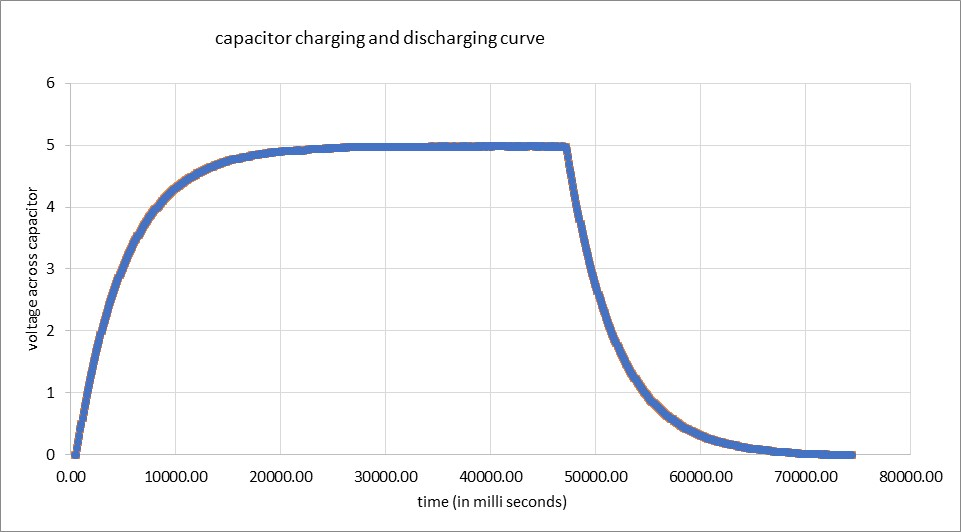
\includegraphics[width=6.14in,height=3.4in]{./media/image4.jpeg}
	\end{Center}
\end{figure}
%%%%%%%%%%%%%%%%%%%% Figure/Image No: 4 Ends here %%%%%%%%%%%%%%%%%%%%

\par

\vspace{\baselineskip}

\vspace{\baselineskip}
{\fontsize{14pt}{16.8pt}\selectfont \textbf{RESULT:\  }\par}\par

{\fontsize{14pt}{16.8pt}\selectfont \textbf{ }\par}\par

{\fontsize{14pt}{16.8pt}\selectfont  This way very easily we can collect data through Arduino where observation of data at each milli seconds is important. This reduces error in observing data as we directly get data from Arduino to excel and observation becomes easy.\par}\par

\vspace{\baselineskip}
{\fontsize{14pt}{16.8pt}\selectfont This type of analysis is useful when more than one circuit components are connected and we have to observe individual components. \par}\par

\vspace{\baselineskip}
{\fontsize{14pt}{16.8pt}\selectfont \ \  \par}\par

\end{document}
